\documentclass[12pt, a4paper]{article}

\usepackage{amsmath}
\usepackage{amssymb}
\usepackage{fontawesome5}

\usepackage{graphicx}
\usepackage{tikz}

\usepackage{hyperref}
\hypersetup{
    colorlinks=false,
    pdfencoding=unicode,
    pdftitle={Reward Machines Comparison},
    pdfauthor={Maximilian Stollmayer},
    pdfpagemode=FullScreen
}


\begin{document}

\section*{Comparison Q-Learning and CRM}

In this little report we will compare the performance of Q-Learning and the CRM algorithm developed for reward machines on a simple environment to see how they differ.

\section*{DoorKey Environment}

The DoorKey environment comes from the minigrid package that builds grid environments compatible with \href{https://gymnasium.farama.org/}{gymnasium}, the reinforcement learning library.

\begin{figure}[h]
	\begin{center}
		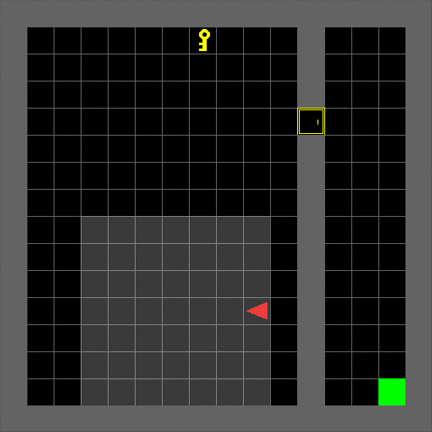
\includegraphics[width=0.5\textwidth]{figures/doorkey.png}
	\end{center}
	\caption{DoorKey environment}
	\label{fig:doorkey}
\end{figure}

The environment consists of an $n \times n$ grid which is separated by a wall with a locked door. The agent starts in one half and in the other half is the exit. In order to reach the exit the agent must pick up a key to unlock the door and get to the other side. Reaching the exit is the goal and upon succeeding the agent is rewarded with 1. If the agent does not reach the goal in a specified number of steps then it is rewarded with 0. See figure \ref{fig:doorkey} for an example of the DoorKey environment.

There are seven available actions for the agent: turning left and right, stepping forward, picking up the key, dropping the key, opening/closing the door and doing nothing. The state the agent receives is its current direction and its field of view, which is a $m \times m$ box in front of the agent facing in the same direction but is blocked by walls. The tiles in the field of view consist of IDs, colors and a possible state, e.g. open, closed and locked for the door. For convenience this state is encoded as a single integer using the MD5 hashing function to make it immediately usable in the algorithms below.

\section*{Q-Learning}

The baseline we want to compare the reward machine implementation against is simple Q-Learning.

The Q-Learning table $Q$ is initialized with uniformly random values in $[0, 1]$ and updated using the Bellman equation
$$ Q(s_t, a_t) \leftarrow (1 - \alpha) \, Q(s_t, a_t) + \alpha \left( r_{t+1} + \gamma \, \max_a Q(s_{t+1}, a) \right), $$
where $s_t$ is the state, $a_t$ the action and $r_t$ the reward at time $t$, $\alpha$ is the learning rate and $\gamma$ the discount factor.

During training the action is selected using $\epsilon$-greedy action selection, where with probability $\epsilon$ a random action is selected and otherwise the the current best action according to table $Q$. Each training episode the $\epsilon$ value is decaying exponentially until it reaches a minimal value by $\epsilon \leftarrow \max(\epsilon_{\min}, \delta \epsilon)$. During testing we only exploit the $Q$ table.

The parameters for our implementation of Q-Learning are the following:
\begin{itemize}
	\item $\alpha = 0.1$
	\item $\gamma = 0.9$
	\item $\epsilon = 1$
	\item $\delta = 0.995$
	\item $\epsilon_{\min} = 0.01$
\end{itemize}

\section*{CRM and Baseline}

In order to use "Q-Learning with counterfactual experiences for reward machines" (CRM) algorithm described in the paper "Reward Machines: Exploiting Reward Function Structure in Reinforcement Learning" from 2022, we need to construct a reward machine. In figure \ref{fig:rm} below you see the reward machine as a diagram with states $u_0$, $u_1$ and $u_2$. Each edge is labeled with the proposition that has to be fulfilled and the reward that the agent is rewarded in that case. The propositional symbols used are
\begin{itemize}
	\item \faKey\ ... agent has picked up the key
	\item \faDoorOpen\ ... door is opened
	\item \faClock\ ... timeout, i.e. maximum number of steps reached
	\item \faSignOut*\ ... exit, i.e. the goal
\end{itemize}
So state $u_0$ basically is the agent trying to aquire the key, $u_1$ trying to open the door and $u_2$ reaching the exit.

\usetikzlibrary{graphs, quotes}
\begin{figure}[h]
	\centering
	\tikz{
	\node[draw, rounded corners, fill=black] (s) at (0, 0) {};
	\node[draw, rounded corners] (u0) at (0, -1) {$u_0$};
	\node[draw, rounded corners] (u1) at (0, -3) {$u_1$};
	\node[draw, rounded corners] (u2) at (0, -5) {$u_2$};
	\node[draw, rounded corners, fill=black] (t0) at (2, -1) {};
	\node[draw, rounded corners, fill=black] (t1) at (2, -3) {};
	\node[draw, rounded corners, fill=black] (t2) at (2, -5) {};
	\node[draw, rounded corners, fill=black] (e) at (0, -7) {};

	\path (u0) edge[loop left] node {($\neg$\faKey$\wedge\neg$\faClock, 0)} (u0);
	\path (u1) edge[loop left] node {(\faKey$\wedge\neg$\faDoorOpen$\wedge\neg$\faClock, 0)} (u1);
	\path (u2) edge[loop left] node {(\faDoorOpen$\wedge\neg$\faSignOut*$\wedge\neg$\faClock, 0)} (u2);
	\graph{
	(s) -> (u0);
	(u0) ->["(\faClock, 0)"] (t0);
	(u0) ->["(\faKey$\wedge\neg$\faClock, 0)", bend right, swap] (u1);
	(u1) ->["($\neg$\faKey$\wedge\neg$\faDoorOpen$\wedge\neg$\faClock, 0)", bend right, swap] (u0);
	(u1) ->["(\faClock, 0)"] (t1);
	(u1) ->["(\faDoorOpen$\wedge\neg$\faClock, 0)", bend right, swap] (u2);
	(u2) ->["($\neg$\faDoorOpen$\wedge\neg$\faSignOut*$\wedge\neg$\faClock, 0)", bend right, swap] (u1);
	(u2) ->["(\faClock, 0)", swap] (t2);
	(u2) ->["(\faSignOut*$\wedge\neg$\faClock, 1)", swap] (e);
	};
	}
	\caption{Reward machine for the DoorKey environment}
	\label{fig:rm}
\end{figure}

The idea of the CRM algorithm is to use the different states of the reward machine to learn from counterfactual experiences, i.e. the $Q$-table is updated for all reward machine states given the current experience $(s_t, a_t, s_{t+1})$ and not just the current one, which should speed up the convergence.

This means that the Q-table is larger than in the simple Q-Learning case. Thus we will also test the Baseline algorithm, which only uses the current reward machine state and no counterfactual experiences, basically Q-learning with a bigger Q-table. Thus we can compare how much more work CRM has to do compared to a smaller Q-table and also how much exactly the counterfactual reasoning increases performance in this environment.

The hyperparameters are the same as in the Q-Learning case.

\section*{Results}

We run Q-Learning, Baseline and CRM algorithms on the $5 \times 5$ DoorKey environment as well as the $6 \times 6$ one for 600 and 6000 episodes respectively. We tracked the training error, i.e. the average temporal difference error $$r_{t+1} + \gamma \, \max_a Q(s_{t+1}, a) - Q(s_t, a_t)$$ over an episode, as well as the total reward for each episode, so in this case either 0 or 1, and the number of steps taken. We repeated this experiment 100 times and plotted the averages below.

\begin{figure}[ht!]
	\centering
	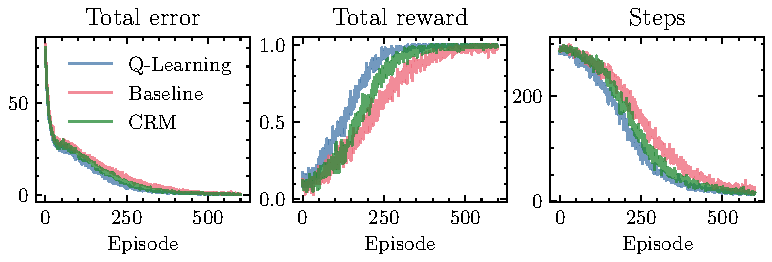
\includegraphics[width=\textwidth]{figures/cmp1_5x5.pdf}
	\caption{Average over 100 runs of the $5 \times 5$ DoorKey environment}
	\label{fig:5x5_1}
\end{figure}

As seen in figure \ref{fig:5x5_1} in roughly the first 400 - 500 episodes the training error fluctuates but settles close to 0 afterwards for all algorithms. Since the total reward can only be 0 or 1 in this case, it can be seen as the percentage of how many runs achieved the goal in that episode. Thus the Q-Learning converges slightly faster to the optimum than both Baseline and CRM, where CRM is slighty better than the Baseline. Similarly Q-Learning also requires less steps on average for each episode. The best and also the median strategy found for all algorithms in these 100 runs takes 11 steps to the exit with only exploiting the learned Q-table. They take this best strategy in 83 - 89 \% of the runs.

\begin{figure}[ht!]
	\centering
	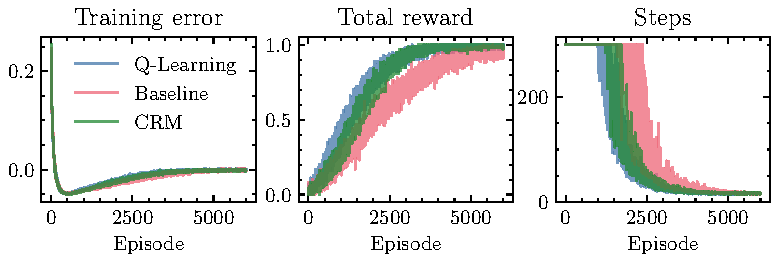
\includegraphics[width=\textwidth]{figures/cmp1_6x6.pdf}
	\caption{Average over 100 runs of the $6 \times 6$ DoorKey environment}
	\label{fig:6x6_1}
\end{figure}

A similar picture can be seen in figure \ref{fig:6x6_1} for the $6 \times 6$ environment, but needed 10 times more episodes to that of the $5 \times 5$ environment. The result is basically the same but with a little more variance. Altough the Baseline algorithm is much slower in convergence. The best strategy for the converged agents takes 14 steps to the exit in all cases, but this is now only taken in 26 - 31 \% of the runs.

\section*{Tuned Results}

Since adjusting the rewards is very easy and intuitive with reward machines we tuned the CRM and Baseline algorithms to improve the convergence. The rewards have been altered in the following way:
\begin{itemize}
	\item picking up the key $\to$ 0.1
	\item dropping key before opening door $\to$ -0.6
	\item opens door $\to$ 0.2
	\item close door $\to$ -0.5
	\item not finishing $\to$ -1
	\item finishing stays at 1
	\item everything else stays at 0
\end{itemize}

\begin{figure}[ht!]
	\centering
	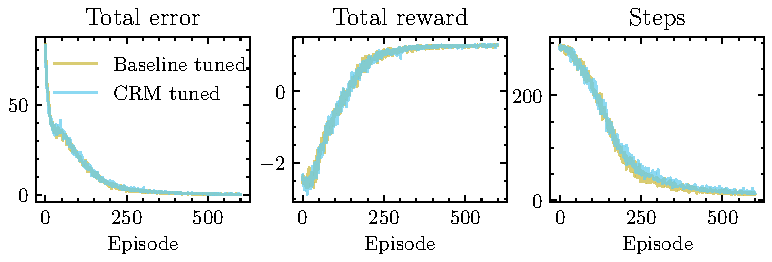
\includegraphics[width=\textwidth]{figures/cmp2_5x5.pdf}
	\caption{Average over 100 runs of the $5 \times 5$ DoorKey environment with tuned reward machines}
	\label{fig:5x5_2}
\end{figure}

\begin{figure}[ht!]
	\centering
	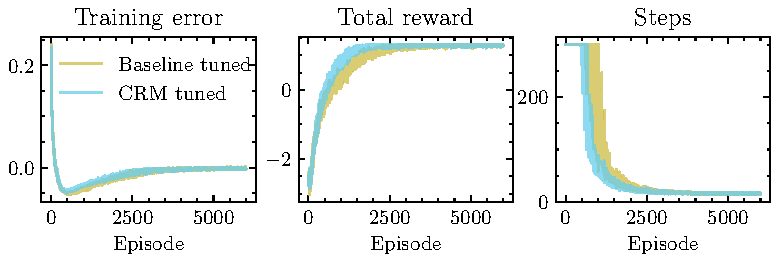
\includegraphics[width=\textwidth]{figures/cmp2_6x6.pdf}
	\caption{Average over 100 runs of the $6 \times 6$ DoorKey environment with tuned reward machines}
	\label{fig:6x6_2}
\end{figure}

For the $5 \times 5$ environment we see in figure \ref{fig:5x5_2} that both tuned reward machines perform very similarly. But figure \ref{fig:6x6_2} shows that CRM converges quicker than the Baseline. They found the same best strategies as the non-tuned algorithms and also take them in a similar portion of runs.

\begin{figure}[ht!]
	\centering
	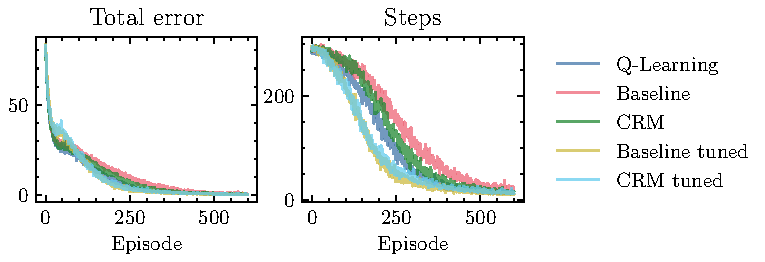
\includegraphics[width=\textwidth]{figures/cmp3_5x5.pdf}
	\caption{Average over 100 runs of the $5 \times 5$ DoorKey environment with tuned reward machines}
	\label{fig:5x5_3}
\end{figure}

\begin{figure}[ht!]
	\centering
	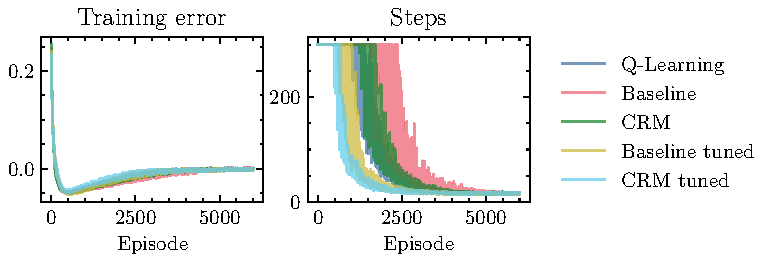
\includegraphics[width=\textwidth]{figures/cmp3_6x6.pdf}
	\caption{Average over 100 runs of the $6 \times 6$ DoorKey environment with tuned reward machines}
	\label{fig:6x6_3}
\end{figure}

In figures \ref{fig:5x5_3} and \ref{fig:6x6_3} we see that both tuned reward machines outperform the non-tuned ones as expected.

\section*{Conclusion}

Altough we would expect CRM to outperform Q-Learning we actually observe that Q-Learning converges a little bit quicker and it also requires fewer steps on average in this environment. An explanation could be that there may not be a lot of repeated states that CRM would benefit from. The additionally updated Q-table entries may not be used and instead the bigger Q-table leads to less refined entries. This could be why there is a gap from Q-Learning to Baseline and CRM is marginally better than Baseline because some but not enough states are hit more than once. This would suggest to repeat these experiments in different environments to see if CRM can close the gap to Q-Learning in them. Also the extension of CRM to Deep Q-Network (DQN) learning should be compare to DQN itself.

\section*{References}

\begin{itemize}
	\item My implementation on \href{https://github.com/maxstollmayer/Reward-Machines}{GitHub}
	\item \href{https://jair.org/index.php/jair/article/view/12440}{Reward Machines: Exploiting Reward Function Structure in Reinforcement Learning} by Rodrigo Toro Icarte, Toryn Q. Klassen, Richard Valenzano and Sheila A. McIlraith
	\item Parts taken from original implementation by Rodrigo Toro Icarte and Toryn Q. Klassen on \href{https://github.com/RodrigoToroIcarte/reward_machines}{GitHub}
	\item \href{https://gymnasium.farama.org/}{Gymnasium} by Farama foundation
	\item \href{https://minigrid.farama.org/environments/minigrid/DoorKeyEnv/}{Minigrid} by Farama foundation
\end{itemize}

\end{document}
